\RequirePackage[]{optional}
%\RequirePackage[slides]{optional}
%\RequirePackage[notslides]{optional}

\opt{slides}{
% Following for presentation mode
\documentclass[10pt]{beamer}
\usepackage{xmpmulti}
%usetheme{Berlin}
}
\opt{notslides}{
% Following for notes mode
\documentclass[a4paper]{article}
\usepackage{beamerarticle}
\usepackage{a4wide}
\usepackage{graphicx}
\usepackage{amsfonts}
\usepackage{fancyhdr}
}

% Following for all modes
%\usepackage{auto-pst-pdf}
%\usepackage{pst-pdf}
\usepackage{psfrag}
\usepackage{setspace}

\parindent=0ex
\parskip=1ex
\newcommand{\conv}{\ast}
\newcommand{\ftpair}{{\stackrel{\cal F}{\longleftrightarrow}}}
\newcommand{\ltpair}{{\stackrel{\cal L}{\longleftrightarrow}}}
\reversemarginpar

%\title{Fourier transform}
%\author{}
%\date{}

\begin{document}
\pagestyle{fancy}
\fancyhead{}
\renewcommand{\headrulewidth}{0pt}
\fancyfoot[C]{\thesection-\thepage}
%\fancyfoot[R]{fcn2010}

\begin{frame}
\titlepage
\end{frame}

\setcounter{section}{6}
\section{Laplace transform}

The Laplace transform is a generalised Fourier transform that can handle a larger class of signals.  Instead of a real-valued frequency variable $\omega$ indexing the exponential component $e^{j \omega t}$ it uses a complex-valued variable $s$ and the generalised exponential $e^{s t}$.  If all signals of interest are right-sided (zero for negative $t$) then a unilateral variant can be defined that is simple to use in practice.  

\subsection{Development}

The Fourier transform of a signal $x(t)$ exists if it is absolutely integrable:
\begin{equation*}
  \int_{-\infty}^{\infty} |x(t)| dt < \infty.
\end{equation*}
While it's possible that the transform might exist even if this condition isn't satisfied, there are a whole class of signals of interest that do not have a Fourier transform.  We still need to be able to work with them.

Consider the signal $x(t) = e^{2t} u(t)$.  For positive values of $t$ this signal grows exponentially without bound, and the Fourier integral does not converge.  However, we observe that the modified signal $\phi(t) = x(t) e^{-\sigma t}$ does have a Fourier transform if we choose $\sigma>2$.  Thus $\phi(t)$ can be expressed in terms of frequency components $e^{j \omega t}$ for $-\infty < \omega < \infty$.  

The bilateral Laplace transform of a signal $x(t)$ is defined to be
\begin{equation*}
  X(s) = \int_{-\infty}^{\infty} x(t) e^{-st} dt,
\end{equation*}
where $s$ is a complex variable.  The set of values of $s$ for which this transform exists is called the {\it region of convergence}, or ROC.   Suppose the imaginary axis $s=j \omega$ lies in the ROC.  The values of the Laplace transform along this line are
\begin{equation*}
  X(j \omega) = \int_{-\infty}^{\infty} x(t) e^{-j \omega t} dt,
\end{equation*}
which are precisely the values of the Fourier transform.

Writing $s = \sigma + j \omega$ this integral can be expanded as
\begin{equation*}
  X(\sigma + j \omega) = \int_{-\infty}^{\infty} x(t) e^{- \sigma t} e^{-j \omega t} dt,
\end{equation*}
which is the Fourier transform of $x(t) e^{- \sigma t}$.  

Since ${\cal F} \{ x(t) e^{- \sigma t} \} = X(\sigma + j \omega)$ the Fourier reconstruction formula gives
\begin{equation*}
  x(t) e^{- \sigma t} = \frac{1}{2\pi} \int_{-\infty}^{\infty} X(\sigma + j \omega) e^{j \omega t} d\omega.
\end{equation*}
Multiplying both sides by $e^{\sigma t}$ yields
\begin{equation*}
  x(t) = \frac{1}{2\pi} \int_{-\infty}^{\infty} X(\sigma + j \omega) e^{(\sigma + j \omega) t} d\omega.
\end{equation*}
With the change of variables $s = \sigma + j \omega$ we have $ds = j d\omega$, and the inverse transform is
\begin{equation*}
  x(t) = \frac{1}{2\pi j} \int_{\sigma-j \infty}^{\sigma+j \infty} X(s) e^{s t} d\omega.
\end{equation*}
This is a line integral in the complex plane.  In practice any value of $\sigma$ can be used that corresponds to a line in the region of convergence.  This integration in the complex plane requires knowledge in theory of functions of complex variables, but in practice we can avoid explicit integration by using tables of Laplace transform pairs.

The Fourier synthesis formula reconstructs a signal using a set of scaled complex exponentials of the form $e^{j \omega t}$ for various values of $\omega$.  For a real-valued signal the positive and negative frequency components can be combined into sinusoids.  The first plot below shows two such reconstruction basis functions for the Fourier transform.  The basis functions for the Laplace transform include an exponential envelope that either increases or decreases with time, and two of these functions are shown in the second plot below.  Since these functions grow with time they can represent signals that grow with time.  This is the reason why the Laplace transform can represent a larger class of signals than the Fourier transform.\begin{center}
  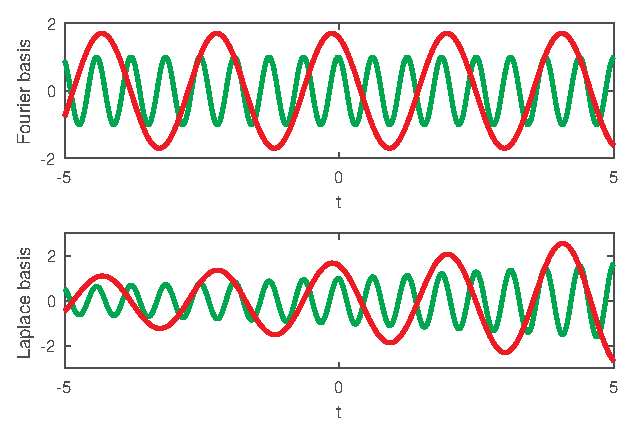
\includegraphics{laplacerecbasis}
\end{center}

The remainder of this section demonstrates how some bilateral Laplace transforms can be calculated.  To continue we will need the following result:
\begin{center}
\fbox{
\begin{minipage}{0.9\textwidth}
With $z = \alpha + j \beta$ we have
\begin{equation*}
  \lim_{t \to \infty} e^{-zt} = \lim_{t \to \infty} e^{-(\alpha + j\beta) t} = \lim_{t \to \infty} e^{-\alpha t} e^{j\beta t}.
\end{equation*}
The quantity $e^{-\alpha t} e^{j\beta t}$ is just a complex number expressed in polar form, with magnitude $e^{-\alpha t}$.  For $\alpha > 0$ this magnitude tends to zero as $t \to \infty$, so in general 
\begin{equation*}
  \lim_{t \to \infty} e^{-zt} = \begin{cases}
    0 \quad & \text{if~} \text{Re}(z) > 0 \\
    \infty \quad & \text{if~} \text{Re}(z) < 0.
  \end{cases}
\end{equation*}
\end{minipage}
}
\end{center}

The Laplace transform of the signal $x(t) = e^{-at} u(t)$ for a possibly complex value $a$ can now be found:
\begin{equation*}
  {\cal L} \{ x(t) \} = X(s) = \int_{-\infty}^{\infty} e^{-at} u(t) e^{-st} dt
  = \int_{0}^{\infty} e^{-(s+a)t} dt = \frac{-1}{s+a} \left[ e^{-(s+a)t} \right]_{t=0}^\infty.
\end{equation*}
Using the above result the transform is therefore
\begin{equation*}
  X(s) = \frac{-1}{s+a} (0-1) = \frac{1}{s+a} \quad \text{with ROC} \quad \text{Re}(s+a) > 0,
\end{equation*}
leading to the Laplace transform pair
\begin{equation*}
  e^{-at} u(t) \quad \Longleftrightarrow \quad \frac{1}{s+a} \qquad \text{Re}(s) > - \text{Re}(a).
\end{equation*}
Note that this holds for all $a$.  However, if $ \text{Re}(a)$ is negative then the transform does not converge on the line $s = j \omega$, and the Fourier transform does not exist.

The region of convergence is a critical component of the Laplace transform.  Using a derivation analogous to the one above we determine that the following is a valid Laplace transform pair:
\begin{equation*}
  -e^{-at} u(-t) \quad \Longleftrightarrow \quad \frac{1}{s+a} \qquad \text{Re}(s) < - \text{Re}(a).
\end{equation*}
The signals $e^{-at} u(t)$ and $-e^{-at} u(-t)$ therefore have the same Laplace transform --- only the ROCs are different.  Thus there is no one-to-one correspondence between $x(t)$ and $X(s)$ unless the ROC is specified, which makes the transform tricky to use.  This ambiguity vanishes if we restrict all our signals to be causal or right-sided.  For example, the Laplace transform $X(s) = 1/(s+a)$ then has only one inverse, namely $e^{-at} u(t)$, and we are not required to know the ROC.  This leads to the {\em unilateral} Laplace transform.

\subsection{Unilateral Laplace transform}

When people talk about the Laplace transform they usually mean the unilateral variant
\begin{equation*}
  X(s) = \int_{0^-}^\infty x(t) e^{-st} dt.
\end{equation*}
This is essentially just the bilateral Laplace transform applied to a signal that is known to be zero for negative time, also called a {\em right-sided} signal.  The lower integration limit is taken to be $0^-$, infinitesimally before $t=0$.  This allows for impulses at the origin, and permits a natural specification of initial conditions when using the transform to solve differential equations.  The unilateral Laplace transform cannot handle signals that are not right-sided, or systems that are not causal.

There is essentially no difference between the unilateral and the bilateral Laplace transform, except that the former deals with the subclass of signals that start at $t=0$.  The inverse transform therefore remains unchanged.

By way of example consider firstly the transform of $\delta(t)$:
\begin{equation*}
  {\cal L}\{ \delta(t) \} = \int_{0^-}^\infty \delta(t) e^{-st} dt =  \int_{0^-}^\infty \delta(t) e^{-s(0)} dt 
  = e^{-s(0)} \int_{0^-}^\infty \delta(t) dt = 1.
\end{equation*}
Thus the following Laplace transform pair is obtained:
\begin{equation*}
  \delta(t) \quad \Longleftrightarrow \quad 1 \qquad \text{for all $s$}.
\end{equation*}
Similarly 
\begin{align*}
  {\cal L}\{ \cos(\omega_0 t) u(t) \} &= {\cal L}\{ 1/2 e^{j \omega_0 t} u(t) + 1/2 e^{-j \omega_0 t} u(t) \} 
  = \frac{1/2}{s-j \omega_0} + \frac{1/2}{s+j \omega_0}
\end{align*}
for $\text{Re}(s) > - \text{Re}(-j \omega_0)$ and $\text{Re}(s) > - \text{Re}(j \omega_0)$, or just $\text{Re}(s)>0$.  Multiplying out yields the Laplace transform pair
\begin{equation*}
  \cos(\omega_0 t) u(t) \quad \Longleftrightarrow \quad \frac{s}{s^2 + \omega_0^2} \qquad \text{for $\text{Re}(s)>0$}.
\end{equation*}
Since for unilateral Laplace transforms any $F(s)$ has a unique inverse, we generally ignore any reference to the ROC.  Note however that finding a Fourier transform by evaluating the Laplace transform at $s=j\omega$ is only valid if the imaginary axis lies in the ROC.

Finding the inverse Laplace transform using the synthesis formula requires integration in the complex plane, which is a subject in its own right.  In practice for the signals of interest we can simply find inverse transforms using tables.  This is because most transforms $F(s)$ that we care about are rational functions of the form $F(s) = P(s)/Q(s)$, where $P(s)$ and $Q(s)$ are polynomials in $s$.  The values of $s$ for which $F(s)=0$ are called the {\em zeros} of $F(s)$, and the values where $F(s) \to \infty$ are the {\em poles} of $F(s)$.  For rational functions the zeros satisfy $P(s)=0$ and the poles satisfy $Q(s)=0$.

The table below contains some common unilateral Laplace transform pairs: 
\begin{center}
\fbox{
\begin{minipage}{0.9\textwidth}
\doublespacing
\begin{center}
\begin{tabular}[h]{ll}
  
  $x(t) = \frac{1}{2\pi j} \int_{c-j\infty}^{c+j\infty} X(s) e^{s t} ds \quad $& 
  $X(s) = \int_{0^-}^{\infty} x(t) e^{-s t} dt$ \\
  \noalign{\vskip 0.5mm} 
  \hline

  $\delta(t)$ &
  $1$ \\

  $u(t)$ &
  $\frac{1}{s}$ \\

  $t u(t)$ &
  $\frac{1}{s^2}$ \\

  $t^n u(t)$ &
  $\frac{n!}{s^{n+1}}$ \\

  $e^{\lambda t} u(t)$ &
  $\frac{1}{s-\lambda}$ \\

  $t e^{\lambda t} u(t)$ &
  $\frac{1}{(s-\lambda)^2}$ \\

  $t^n e^{\lambda t} u(t)$ &
  $\frac{n!}{(s-\lambda)^{n+1}}$ \\

  $\cos(bt) u(t)$ &
  $\frac{s}{s^2+b^2}$ \\

  $\sin(bt) u(t)$ &
  $\frac{b}{s^2+b^2}$ \\
  
  $e^{-at} \cos(bt) u(t)$ &
  $\frac{s+a}{(s+a)^2+b^2}$ \\

  $e^{-at} \sin(bt) u(t)$ &
  $\frac{b}{(s+a)^2+b^2}$ \\

  $r e^{-a t} \cos(bt + \theta) u(t)$ &
  $\frac{(r \cos \theta) s + (a r \cos \theta - b r \sin \theta) }{s^2 + 2 a s + (a^2 + b^2)}$ \\

  $r e^{-a t} \cos(bt + \theta) u(t)$ &
  $\frac{0.5 r e^{j \theta}}{s + a - jb} + \frac{0.5 r e^{-j \theta}}{s + a + jb}$ \\

  $r e^{-a t} \cos(bt + \theta) u(t)$ &
  $\frac{A s + B}{s^2 + 2 a s + c}$ \\
  
  $$ & $r = \sqrt{\frac{A^2 c + B^2 - 2 A B a}{c-a^2}}$, $b = \sqrt{c-a^2}$, $\theta = \tan^{-1} \frac{A a - b}{A \sqrt{c-a^2}}$ \\

  \noalign{\vskip 0.5mm}
\end{tabular}
\end{center}
\end{minipage}
}
\end{center}

Suppose for example we wanted to find the right-sided inverse transform of 
\begin{equation*}
  F(s) = \frac{8s+10}{(s+1)(s+2)^3}.
\end{equation*}
This has a zero at $s=-10/8 = -5/4$, a pole at $s=-1$, and a pole of order three (or three poles) at $s=-2$.

Using partial fractions we can write
\begin{equation*}
  \frac{8s+10}{(s+1)(s+2)^3} = \frac{2}{s+1} + \frac{6}{(s+2)^3} - \frac{2}{(s+2)^2} - \frac{2}{s+2}.
\end{equation*}
From tables the Laplace transform pair
\begin{equation*}
  t^n e^{\lambda t} u(t) \quad \Longleftrightarrow \quad \frac{n!}{(s-\lambda)^{n+1}}
\end{equation*}
can then be used to obtain the inverse transform
\begin{equation*}
  f(t) = [ 2e^{-t} + (3 t^2 - 2 t - 2) e^{-2 t} ] u(t). 
\end{equation*}

{\em Convince
\marginpar{\bf Exercise:} 
yourself that the form of the partial fraction expansion above is appropriate, derive the values for the coefficients, and verify the inverse transform.}

\subsection{Laplace transform properties}

Since the bilateral Laplace transform is a generalised Fourier transform we would expect many of the properties to be similar, and this is indeed the case.  However, the properties of the unilateral Laplace transform are slightly different and require explanation.

A summary of the Laplace transform properties appears below.  In all cases we assume that $x(t) \ftpair X(s)$ and $v(t) \ftpair V(s)$ are valid transform pairs.  
\begin{center}
\fbox{
\begin{minipage}{0.9\textwidth}
\doublespacing
\begin{tabular}[h]{ll}
  %\hline
  Property \hspace*{20ex} & Transform Pair/Property \\
  \hline

  Linearity &
  $a x(t) + b v(t) \Longleftrightarrow a X(s) + b V(s)$ \\
  
  Time shift &
  $x(t-a) u(t-a) \Longleftrightarrow e^{-as} X(s) \quad a \geq 0$ \\

  Time scaling &
  $x(at) \Longleftrightarrow \frac{1}{a} X(\frac{s}{a}) \quad a > 0$ \\

 % Time reversal &
 % $x(-t) \Longleftrightarrow X(-\omega) = \overline{X(\omega)}$ \\

  Frequency differentiation &
  $t^n x(t) \Longleftrightarrow (-1)^n X^{(n)}(s)$ \\

  Frequency shift &
  $e^{a t} x(t) \Longleftrightarrow X(s - a)$ \\

 % Multiplication by $\cos(\omega_0 t)$ &
 % $x(t) \cos(\omega_0 t) \Longleftrightarrow \frac{1}{2} [ X(\omega +
 % \omega_0) + X(\omega - \omega_0) ]$ \\

  Differentiation &
  $x'(t) \Longleftrightarrow s X(s) - x(0^-)$ \\

  &
  $x''(t) \Longleftrightarrow s^2 X(s) - s x(0^-) - x'(0^-)$ \\
  
  &
  $x^{(n)}(t) \Longleftrightarrow s^n X(s) - s^{n-1} x(0^-) - \cdots - x^{(n-1)}(0^-)$ \\

  Integration &
  $\int_{0^-}^t x(\lambda) d\lambda \Longleftrightarrow \frac{1}{s} X(s)$ \\

  &
  $\int_{-\infty}^t x(\lambda) d\lambda \Longleftrightarrow \frac{1}{s} X(s) + 
  \frac{1}{s} \int_{-\infty}^{0^-} x(\lambda) d\lambda$ \\

  Time convolution &
  $x(t) \conv v(t) \Longleftrightarrow X(s) V(s)$ \\

 Frequency convolution &
 $x(t) v(t) \Longleftrightarrow \frac{1}{2\pi j} X(s) \conv V(s)$ \\

  %\hline
\end{tabular}
\end{minipage}
}
\end{center}
The properties are exposed in more detail in the remainder of this section.

\subsubsection{Time shift}
Suppose we have a valid unilateral Laplace transform pair $x(t) u(t) \ltpair X(s)$.  The transform of the signal shifted to the right is then
\begin{equation*}
  {\cal L} \{ x(t-t_0) u(t-t_0) \} = \int_{0^-}^\infty x(t-t_0) u(t-t_0) e^{-st} dt
  = \int_{(-t_0)^-}^\infty x(p) u(p) e^{-s(p+t_0)} dp,
\end{equation*}
where the change of variables $p = t-t_0$ has been made.  If $t_0<0$ then the shifted signal is no longer right-sided and the unilateral Laplace transform is inappropriate, so we require $t_0>0$.  Under these conditions, since $u(p)=0$ for $p<0$ the lower integration limit can be changed from $(-t_0)^-$ to $0^-$, yielding
\begin{equation*}
  {\cal L} \{ x(t-t_0) u(t-t_0) \} = \int_{0^-}^\infty x(p) u(p) e^{-s(p+t_0)} dp = 
  e^{-s t_0} \int_{0^-}^\infty x(p) u(p) e^{-s p} dp = e^{-s t_0} X(s).
\end{equation*}

The resulting property is as follows:
\begin{center}
\fbox{
\begin{minipage}{0.9\textwidth}
Time shift:
\begin{align*}
  \text{If} \quad x(t) & \ltpair X(s) \\
  \text{then} \quad x(t-t_0) \quad & \ltpair \quad e^{-s t_0} X(s) \quad \text{for $t_0>0$}.
\end{align*}
\end{minipage}
}
\end{center}

\subsubsection{Scaling}

If $x(t) \ltpair X(s)$ then for $a>0$ we have
\begin{equation*}
  {\cal L} \{ x(at) \} = \int_{0^-}^\infty x(at) e^{-s t} dt
  = \int_{0^-}^\infty x(p) e^{-\frac{s}{a} p} \frac{1}{a} dp = \frac{1}{a} X \left( \frac{s}{a} \right),
\end{equation*}
with $p=at$.  The property is summarised as follows:
\begin{center}
\fbox{
\begin{minipage}{0.9\textwidth}
Scaling:
\begin{align*}
  \text{If} \quad x(t) & \ltpair X(s) \\
  \text{then} \quad x(a t) \quad & \ltpair \quad \frac{1}{a} X\left(\frac{s}{a}\right) \quad \text{for $a>0$}.
\end{align*}
\end{minipage}
}
\end{center}

\subsubsection{Frequency shift}
If $x(t) \ltpair X(s)$ then
\begin{equation*}
  {\cal L} \{ x(t) e^{s_0 t} \} = \int_{0^-}^\infty x(t) e^{s_0 t} e^{-s t} dt
  = \int_{0^-}^\infty x(t) e^{-(s-s_0) t} dt = X(s-s_0).
\end{equation*}
The property is summarised as follows:
\begin{center}
\fbox{
\begin{minipage}{0.9\textwidth}
Frequency shift:
\begin{align*}
  \text{If} \quad x(t) & \ltpair X(s) \\
  \text{then} \quad x(t) e^{s_0 t} \quad & \ltpair \quad X(s-s_0).
\end{align*}
\end{minipage}
}
\end{center}
Note the symmetry or duality between this and the time shift property.

\subsubsection{Time differentiation}
Consider the Laplace transform of the derivative $dx(t)/dt$ of a signal $x(t)$ for which $x(t) \ltpair X(s)$:
\begin{equation*}
  {\cal L} \left\{ \frac{dx}{dt} \right\} = \int_{0^-}^\infty \frac{dx}{dt} e^{-st} dt.
\end{equation*}
Using integration by parts gives
\begin{equation*}
   {\cal L} \left\{ \frac{dx}{dt} \right\} = \left[ x(t) e^{-st} \right]_{t=0^-}^\infty 
   + s \int_{0^-}^\infty x(t) e^{-st} dt.
\end{equation*}
For the Laplace transform to converge we must have $x(t) e^{-s t} \to 0$ as $t \to \infty$ for values of $s$ in the ROC of $X(s)$, in which case
\begin{equation*}
   {\cal L} \left\{ \frac{dx}{dt} \right\} = -x(0^-) + s X(s).
\end{equation*}
This property can be repeatedly applied to give Laplace transforms of higher-order derivatives.

A summary of the property follows.  The quantity $\dot{x}(t)$ indicates the first derivative of $x(t)$ with respect to time, and $x^{(n)}(t)$ indicates the $n$th derivative.
\begin{center}
\fbox{
\begin{minipage}{0.9\textwidth}
Time differentiation:
\begin{align*}
  \text{If} \quad x(t) & \ltpair X(s) \\
  \text{then} \quad \frac{dx}{dt} \quad \ltpair \quad s X(s) - x(0^-) \quad & \text{and} \quad
  \frac{d^2 x}{dt^2} \quad \ltpair \quad s^2 X(s) - s x(0^-) - \dot{x}(0^-). 
\end{align*}
In general
\begin{equation*}
  \frac{d^n x}{dt^n} \quad \ltpair \quad s^n X(s) - s^{n-1} x(0^-) - s^{n-2} \dot{x}(0^-) - \cdots - x^{(n-1)}(0^-).
\end{equation*}

\end{minipage}
}
\end{center}

\subsubsection{Time integration}

Suppose $f(t) \ltpair F(s)$ and $g(t) \ltpair G(s)$.  If we define 
\begin{equation*}
  g(t) = \int_{0^-}^t f(\tau) d\tau
\end{equation*}
then $f(t) = \frac{dg(t)}{dt}$ and $g(0^-) = 0$.  Now
\begin{equation*}
  F(s) = {\cal L} \left\{ \frac{d}{dt} g(t) \right\} = s G(s) - g(0^-) = s G(s),
\end{equation*}
so $G(s) = F(s)/s$.  Thus
\begin{equation*}
  \int_{0^-}^t f(\tau) d\tau \quad \ltpair \quad \frac{F(s)}{s}.
\end{equation*}

The property is as follows:
\begin{center}
\fbox{
\begin{minipage}{0.9\textwidth}
Time integration:
\begin{gather*}
  \text{If} \quad x(t) \ltpair X(s) \\
  \text{then} \quad \int_{0^-}^t x(\tau) d\tau \quad \ltpair \quad \frac{X(s)}{s} \quad \text{and}
  \quad \int_{-\infty}^t x(\tau) d\tau \quad \ltpair \quad \frac{X(s)}{s} + \frac{\int_{-\infty}^{0^-} x(\tau) d\tau}{s}.
\end{gather*}
\end{minipage}
}
\end{center}

\subsubsection{Convolution}

Suppose $f_1(t) \ltpair F_1(s)$ and $f_2(t) \ltpair F_2(s)$.  Then
\begin{align*}
  {\cal L} \{ f_1(t) \conv f_2(t) \} &= {\cal L} \left\{ \int_{0^-}^\infty f_1(\lambda) f_2(t-\lambda) d\lambda \right\}
  =  \int_{0^-}^\infty \left[ \int_{0^-}^\infty f_1(\lambda) f_2(t-\lambda) d\lambda \right] e^{-st} dt \\
  &=  \int_{0^-}^\infty f_1(\lambda) \left[ \int_{0^-}^\infty f_2(t-\lambda) e^{-st} dt \right] d\lambda
  =  \int_{0^-}^\infty f_1(\lambda) \left[ \int_{0^-}^\infty f_2(u) e^{-s(u+\lambda)} du \right] d\lambda \\
  &=  \int_{0^-}^\infty f_1(\lambda) \left[ e^{-s \lambda} \int_{0^-}^\infty f_2(u) e^{-s u} du \right] d\lambda
  =  \int_{0^-}^\infty f_1(\lambda) e^{-s \lambda} d\lambda \int_{0^-}^\infty f_2(u) e^{-s u} du \\
  &= F_1(s) F_2(s).
\end{align*}
Thus convolution in time is equivalent to multiplication of Laplace transforms.  Additionally it can be shown that multiplication in time corresponds to convolution in the Laplace domain.  These properties can be summarised as follows:
\begin{center}
\fbox{
\begin{minipage}{0.9\textwidth}
Convolution:
\begin{gather*}
  \text{If} \quad x(t) \ltpair X(s) \quad \text{and} \quad v(t) \ltpair V(s) \\
  \text{then} \quad x(t) \conv v(t) \quad \ltpair \quad X(s) V(s) \quad \text{and} 
  \quad x(t) v(t) \quad \ltpair \quad \frac{1}{2 \pi j} [X(s) \conv V(s)].
\end{gather*}
\end{minipage}
}
\end{center}

\subsubsection{Initial and final values}

One often needs to know the value of $f(t)$ as $t \to 0$ and $t \to \infty$, the initial and final values.  If you have the Laplace transform then it's not necessary to obtain the inverse transform to find these values.

Since $df/dt \ltpair s F(s) - f(0^-)$ we have
\begin{align*}
  s F(s) - f(0^-) &= \int_{0^-}^\infty \frac{df}{dt} e^{-st} dt
  = \int_{0^-}^{0^+} \frac{df}{dt} e^{-st} dt + \int_{0^+}^\infty \frac{df}{dt} e^{-st} dt \\
  &= \int_{0^-}^{0^+} \frac{df}{dt} e^{0} dt + \int_{0^+}^\infty \frac{df}{dt} e^{-st} dt
  = f(0^+) - f(0^-) + \int_{0^+}^\infty \frac{df}{dt} e^{-st} dt.
\end{align*}
Thus 
\begin{equation*}
  \lim_{s \to \infty} s F(s) = f(0^+) + \lim_{s \to \infty} \int_{0^+}^\infty \frac{df}{dt} e^{-st} dt
  = f(0^+) + \int_{0^+}^\infty \frac{df}{dt} \left( \lim_{s \to \infty} e^{-st} \right) dt = f(0^+).
\end{equation*}
The following is a statement of the property:
\begin{center}
\fbox{
\begin{minipage}{0.9\textwidth}
Initial value:
\begin{gather*}
  \text{If $f(t)$ and its derivative $\frac{df}{dt}$ are both Laplace transformable then} \\
  f(0^+) = \lim_{s \to \infty} s F(s) \qquad \text{if the limit exists.}
\end{gather*}
\end{minipage}
}
\end{center}

Also, since 
\begin{equation*}
  \lim_{s \to 0} [s F(s) - f(0^-)] = \lim_{s \to 0} \int_{0^-}^\infty \frac{df}{dt} e^{-st} dt
  = \int_{0^-}^\infty \frac{df}{dt}dt = \left. f(t) \right|_{0^-}^\infty = \lim_{t \to \infty} f(t) - f(0^-),
\end{equation*}
we have the following property:
\begin{center}
\fbox{
\begin{minipage}{0.9\textwidth}
Final value:
\begin{gather*}
  \text{If $f(t)$ and its derivative $\frac{df}{dt}$ are both Laplace transformable then} \\
  \lim_{t \to \infty} f(t) = \lim_{s \to 0} s F(s) \qquad \text{as long as all poles are in the left half plane.}
\end{gather*}
\end{minipage}
}
\end{center}

\subsection{Solutions of differential equations}

The time-differentiation Laplace transform property $d^k y/dt^k \Longleftrightarrow s^k Y(s)$ can be used to solve linear constant coefficient differential equations with arbitrary input conditions.  Essentially, the transform turns the differential equation into an algebraic equation that is readily solved for $Y(s)$, and the inverse is then the solution $y(t)$.

Suppose we want to find the solution to the differential equation
\begin{equation*}
  \frac{d^2 y(t)}{dt^2} - 4 y(t) = x(t)
\end{equation*}
for $x(t) = \sin(2t) u(t)$ and under the initial conditions $y(0^-)=1$ and $y'(0^-)=-2$.  This is called an {\em initial value problem}, or IVP.

Using the derivative property we have
\begin{equation*}
  \frac{d^2 y(t)}{dt^2} \quad \ltpair \quad s^2 Y(s) - s y(0^-) - y'(0^-).
\end{equation*}
The differential equation in the transform domain therefore becomes
\begin{equation*}
  s^2 Y(s) - s y(0^-) - y'(0^-) - 4 Y(s) = X(s),
\end{equation*}
or
\begin{equation*}
  Y(s) = \frac{X(s)}{s^2-4} + \frac{s y(0^-) + y'(0^-)}{s^2-4}.
\end{equation*}
For the particular problem under consideration we can find the transform of $x(t)$ as
\begin{equation*}
  \sin(2t) u(t) \quad \ltpair \quad \frac{2}{s^2 + 4},
\end{equation*}
and substitute for $X(s)$ and the initial values.  The required solution in the Laplace transform domain is then found to be
\begin{equation*}
  Y(s) = \frac{2}{(s^2+4)(s^2-4)} + \frac{s-2}{s^2-4} = \frac{2}{(s^2+4)(s+2)(s-2)} + \frac{1}{s+2}.
\end{equation*}
The time-domain solution is obtained by finding the inverse transform.  Using partial fractions we can write
\begin{equation*}
  \frac{2}{(s^2+4)(s+2)(s-2)} = \frac{-1/4}{s^2+4} + \frac{-1/16}{s+2} + \frac{1/16}{s-2},
\end{equation*}
so
\begin{equation*}
  y(t) = -1/8 \sin(2 t) u(t) + 15/16 e^{-2 t} u(t) + 1/16 e^{2 t} u(t).
\end{equation*}

The expression obtained earlier, namely 
\begin{equation*}
  Y(s) = \frac{X(s)}{s^2-4} + \frac{s y(0^-) + y'(0^-)}{s^2-4},
\end{equation*}
is interesting.  We can distinguish between two cases.  When $x(t)$ (or $X(s)$) is zero then the solution satisfies
\begin{equation*}
  Y(s) = \frac{s y(0^-) + y'(0^-)}{s^2-4}.
\end{equation*}
This is called the {\em zero-input} component, and its solution is called the zero-input response $y_{zi}(t)$.  This response is independent of the forcing function or input $x(t)$, and essentially characterises how the system responds to the initial conditions.  On the other hand, when the initial conditions $y(0^-)$ and $y'(0^-)$ are zero then the resulting solution satisfies
\begin{equation*}
  Y(s) = \frac{X(s)}{s^2-4}.
\end{equation*}
for the given $X(s)$.  This is called the {\em zero-state} component and its solution is the zero-state response $y_{zs}(t)$.  Saying that the initial value and derivates are all zero prior to the application of the input is exactly the initial rest conditions that were discussed when dealing the the Fourier transform.  Since we can write this last equation as
\begin{equation*}
  Y(s) = \frac{1}{s^2-4} X(s) = H(s) X(s)
\end{equation*}
for $H(s)= \frac{1}{s^2-4}$ we see that this component of the solution satisfies $y_{zs}(t) = h(t) \conv x(t)$, where $h(t)$ is the impulse response of the system under the initial rest conditions.  The total solution to the differential equation is the sum of these two responses $y(t) = y_{zs}(t) + y_{zi}(t)$.  The decomposition of the solution into these two components is similar but not directly related to the decomposition into homogeneous and particular solutions you may have encountered before.

Applying this decomposition directly to the problem described before we see that the two components of the solution are
\begin{equation*}
  y_{zs}(t) = -1/8 \sin(2 t) u(t) - 1/16 e^{-2 t} u(t) + 1/16 e^{2 t} u(t) \qquad \text{and} \qquad y_{zi}(t) = e^{-2t} u(t).
\end{equation*}
\begin{center}
  \psfrag{t}{\scriptsize $t$}
  \psfrag{yzs(t)}{\scriptsize $y_{zs}(t)$}
  \psfrag{yzi(t)}{\scriptsize $y_{zi}(t)$}
  \psfrag{y(t)}{\scriptsize $y(t)$}
  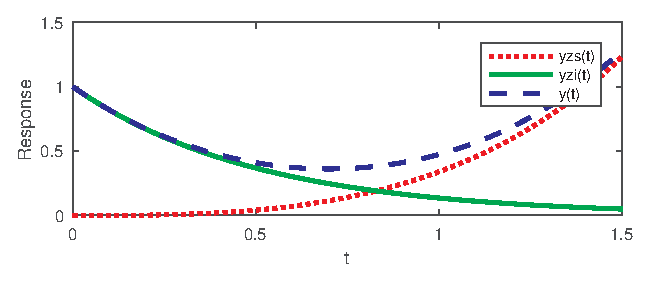
\includegraphics{lapdezizs}
\end{center}
We can note that the zero-state solution (and therefore the total solution) grows without bound, even though the input is bounded.  Any system corresponding to this differential equation is therefore unstable, but the Laplace transform still handles it correctly.  We could also evaluate the stability of the system by noting that it has two poles, one at $s=-2$ and one at $s=+2$.  All the poles of a stable system lie in the left half-plane, so the presence of this latter pole indicates instability.

\subsection{Circuit response}

The Laplace transform can be used for circuit analysis under general initial conditions.  Consider the circuit below
\begin{center}
  \psfrag{Va=5V}{\scriptsize $V_a=5$V}
  \psfrag{vR(t)}{\scriptsize $v_R(t)$}
  \psfrag{vL(t)}{\scriptsize $v_L(t)$}
  \psfrag{vC(t)}{\scriptsize $v_C(t)$}
  \psfrag{i(t)}{\scriptsize $i(t)$}
  \psfrag{R}{\scriptsize $R$}
  \psfrag{L}{\scriptsize $L$}
  \psfrag{C}{\scriptsize $C$}
  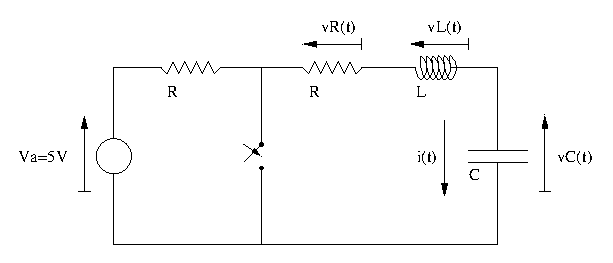
\includegraphics{circuitexlaptr}
\end{center}
with $L=1$H, $R=800\Omega$, and $C=\frac{1}{4.1} \times 10^{-5}$F.  
Suppose that the switch has been open for a very long time and is then closed at $t=0$, and we want to determine a time-domain expression for the subsequent current $i(t)$.  Prior to closing the switch there is no current through the capacitor, so $i(0^-) = 0$A.  Also, since the current is zero and unchanging there is no voltage drop across either of the resistors or the inductor, so $v_C(0^-) = 5$V.  These values specify the initial conditions.  When the switch is closed the voltage source and the resistor on the left have no further effect, and the current that we calculate will show how the capacitor discharges through the resistor-inductor combination.

Kirchhoff's voltage law in the time domain requires that
\begin{equation*}
  v_R(t) + v_L(t) + v_C(t) = 0.
\end{equation*}
To continue we need to consider the voltage-current relationships for each device.  For the resistor and the inductor we have
\begin{equation*}
  v_R(t) = R i(t) \qquad \text{and} \qquad v_L(t) = L \frac{di(t)}{dt}.
\end{equation*}
The capacitor is a little more complicated.  It satisfies
\begin{equation*}
  i(t) = C \frac{dv_C(t)}{dt} \qquad \text{or} \qquad \frac{dv_C(t)}{dt} = \dot{v}_C(t) = \frac{1}{C} i(t).
\end{equation*}
In general if we know $v_C(0)$ then for positive $t$ we can express $v_C(t)$ using the fundamental theorem of calculus:
\begin{equation*}
  v_C(t) = v_C(0^-) + \int_{0^-}^t \dot{v}_C(\tau) d\tau = v_C(0^-) + \frac{1}{C} \int_{0^-}^t i(\tau) d\tau.
\end{equation*}
Substituting into the voltage constraint relationship gives the integro-differential equation
\begin{equation*}
  R i(t) + L \frac{di(t)}{dt} + v_C(0^-) + \frac{1}{C} \int_{0^-}^t i(\tau) d\tau = 0.
\end{equation*}

To solve this equation we apply the Laplace transform, with $i(t) \ltpair I(\omega)$.  The only complicated term involves the inductor, and introduces an initial condition on the current:
\begin{equation*}
  {\cal L} \left\{ L \frac{di(t)}{dt} \right\} = L [s I(s) - i(0^-)].
\end{equation*}
Noting that $v_c(0^-)$ is constant the full transformation is given by
\begin{equation*}
  R I(s) + L [s I(s) - i(0^-)] + \frac{v_C(0^-)}{s} + \frac{I(s)}{sC} = 0,
\end{equation*}
which can be solved for $I(s)$:
\begin{equation*}
  I(s) = \frac{s i(0^-) - \frac{v_c(0^-)}{L}}{s^2 + \frac{R}{L}s + \frac{1}{LC}}.
\end{equation*}

Substituting for all the values for the components and the initial conditions and completing the square gives
\begin{equation*}
  I(s) = \frac{-5}{s^2 + 800 s + 410000} = \frac{-5}{(s+400)^2 + 500^2}.
\end{equation*}
The inverse transform can be obtained by applying the frequency shift property $e^{a t} x(t) \ltpair X(s-a)$ to the Laplace transform pair for the signal $\sin(b t) u(t)$, yielding
\begin{equation*}
  e^{-at} \sin(b t) u(t) \quad \Longleftrightarrow \quad \frac{b}{(s+a)^2 + b^2}.
\end{equation*}
Thus the desired result is
\begin{equation*}
  i(t) = -0.01 e^{-400t} \sin(500 t) u(t).
\end{equation*}

For fixed $L$, if $R$ is increased to a sufficiently large value or if $C$ is decreased then the solution will not be oscillatory --- the damping effect of the resistor dominates the response.  In particular, from the general properties of second-order systems presented later the solution in this case only oscillates if $R<2/\sqrt{C}$, or $C<4/R^2$.  If for example we change the capacitance to $C = (16/3)/ R^2) \approx 8.333 \times 10^{-6}$F then the current is
\begin{equation*}
  I(s) = \frac{-5}{s^2 + R s + \frac{16}{3 R^2}} = \frac{-5}{s + 800 + 120000}
  = \frac{-5}{(s + 600)(s+200)}.
\end{equation*}
Using partial fractions this becomes
\begin{equation*}
  I(s) = \frac{1/80}{s + 600} - \frac{1/80}{s + 200}
\end{equation*}
and the time-domain response is seen to be
\begin{equation*}
  i(t) = \left[ \frac{1}{80} e^{-600 t} - \frac{1}{80} e^{-200 t} \right] u(t).
\end{equation*}

The solutions presented above for the two different cases have very different characteristics.  In the first case the resistance was low enough that the energy could "slosh around" between the capacitor and the inductor before decaying to the steady state.  Hence the sinusoidal solution, decaying as energy is dissipated in the resistor.  In the second case the resistance is high enough that the energy in the capacitor is dissipated before the current reverses direction.  No oscillation occurs and the response is two simple real exponential functions.

The differences in behaviour can be related to the locations of the system poles.  In the first instance the poles must satisfy $(s+400)^2 + 500^2 = 0$, which has the two solutions $s = -400 \pm j 500$.  These poles are complex conjugates of one another; for a real-valued signal poles always occur in conjugate pairs.  The time-domain solution is oscillatory because the poles are complex.  We observe that the real part of this pole pair leads to the exponential factor $e^{-400 t}$, and the imaginary part leads to the oscillation component $\sin(500 t)$.  As the two poles move towards the imaginary axis the rate of decay will decrease and the duration of the response in the time domain will increase.  As the poles move away from the real axis the frequency of the oscillation increases.  In contrast, in the second case the poles are at the real values $s=-600$ and $s=-200$.  These have a zero imaginary component and there is no oscillation.

In the example given above the capacitor had an initial charge, and the circuit differential equation had to be reformulated accordingly.  In practice we usually formulate our circuit equations directly in the Laplace transform domain with complex impedances.  One can deal with the initial conditions by inserting current or voltage generators at appropriate points in the circuit, and then assuming that the active elements are initially at rest.

Take for example the capacitor with governing equation
\begin{equation*}
  i_c(t) = C \frac{d v_C(t)}{dt},
\end{equation*}
which in the transform domain becomes
\begin{equation*}
  I_C(s) = C \left[ s V_C(s) - v_C(0^-) \right].
\end{equation*}
This can be written in two different ways, leading to two different formulations:
\begin{equation*}
  V_C(s) = \frac{1}{Cs} I_C(s) + \frac{v_C(0^-)}{s} \qquad \text{or} \qquad
  V_C(s) = \frac{1}{Cs} [ I_C(s) + C v_C(0^-)].
\end{equation*}
Equivalent circuits for each case are shown below:
\begin{center}
  \psfrag{C}{\scriptsize $C$}
  \psfrag{v(t)}{\scriptsize $v(t)$}
  \psfrag{v(0)}{\scriptsize $v(0)$}
  \psfrag{i(t)}{\scriptsize $i(t)$}
  \psfrag{1/Cs}{\scriptsize $\frac{1}{Cs}$}
  \psfrag{V(s)}{\scriptsize $V(s)$}
  \psfrag{I(s)}{\scriptsize $I(s)$}
  \psfrag{v(0)/s}{\scriptsize $\frac{v(0)}{s}$}
  \psfrag{Cv(0)}{\scriptsize $C v(0)$}
  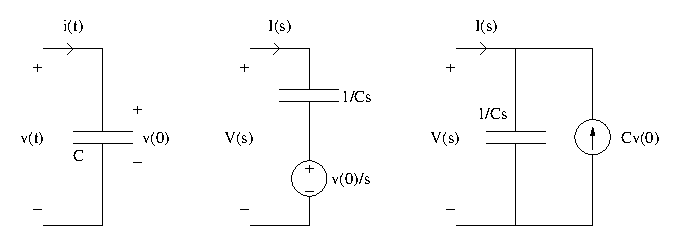
\includegraphics{laplacecapinit}
\end{center}
On the left is the circuit element in the time domain, with an initial charge on the capacitor.  According to the first equation above the voltage-current relationship can be expressed as an initially-discharged capacitor in series with a voltage source with potential $v_c(0)$.  This is demonstrated in the Laplace domain by the equivalent circuit in the center of the figure above.  Alternatively, using the second equation the equivalent circuit looks like an initially-discharged capacitor being driven by a current $I_C(s) + C v_C(0^-)$, depicted on the right-hand side of the figure.  In practice, any time we have a nonzero initial charge on the capacitor we can replace it with an equivalent initial-rest configuration by adding either a constant voltage or current source, which can be thought of as initial condition generators.

{\em The\marginpar{\bf Exercise:} same approach can be used for inductors, which satisfy the time-domain relation $v_L(t) = L d i_L(t)/dt$, under the condition where the initial current is nonzero.  Find the corresponding equivalent circuits using both voltage and current sources.}

\subsection{Feedback and control}

We often want to drive a physical system so that it reaches a desired state.  For example, the cruise control on a car must adjust the engine power until a desired speed is achieved.  This cannot be done by simply modelling the relationship between engine power and car speed, since this relationship will change for example when we go up a hill or when there are more people in the car.  A better approach is to monitor the current speed of the car, and develop a system that will constantly determine the current engine power needed to get the car to this speed and then keep it there.   The input to the system is therefore constantly adjusted to obtain the desired response.  The difference between the actual speed and the desired speed is used as {\em feedback}, and when used appropriately leads to a {\em closed-loop} system.

The remainder of this section uses an example of position control of a rotating system.  This could for example represent the problem of rotating a directional antenna so that it points in a desired direction, or any other problem where a servo-motor is required.  We assume that the object to be rotated has significant rotational inertia $J$, and that there is a viscous damping component $B$ that dissipates the applied torque.  The figure below depicts the system.
\begin{center}
  \psfrag{if}{\scriptsize $i_f$}
  \psfrag{f(t)}{\scriptsize $f(t)$}
  \psfrag{th(t)}{\scriptsize $\theta(t)$}
  \psfrag{J}{\scriptsize $J$}
  \psfrag{B}{\scriptsize $B$}
  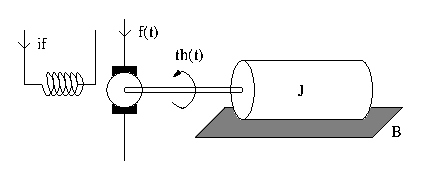
\includegraphics{poscontroldcmotor}
\end{center}
We need a nominal physical model of how the system behaves.  The angle $\theta(t)$ of the rotor is considered to be the output, and can be varied by changing the current $f(t)$ in the motor armature.  Details are as follows.  The motor current $f(t)$ generates a torque $\tau(t) = K_T f(t)$, where $K_T$ is a constant for the motor.  The equivalent of Newton's second law for rotating systems says that applied torque and rotational acceleration are related by $\tau(t) = J \ddot{\theta}(t)$.  The damping component is proportional to angular velocity and reduces torque by $B \dot{\theta}(t)$.  The input $f(t)$ and the output $\theta(t)$ therefore obeys the differential equation
\begin{equation*}
  J \ddot{\theta}(t) = K_T f(t) - B \dot{\theta}(t), \qquad \text{or} \qquad J \ddot{\theta}(t) + B \dot{\theta}(t) = K_T f(t).
\end{equation*}

The Laplace transform of this differential equation is
\begin{equation*}
  J s^2 \Theta(s) + B s \Theta(s) = K_T F(s), \qquad \text{or} \qquad 
  s^2 \Theta(s) + \frac{B}{J} s \Theta(s) = \frac{K_T}{J} F(s).
\end{equation*}
For clarity we assume now that $B/J = 8$ and $K_T/J = 1$.   Since $s^2 \Theta(s) + 8 s \Theta(s) = F(s)$ the transfer function of the system is found to be
\begin{equation*}
  G(s) = \frac{\Theta(s)}{F(s)} = \frac{1}{s(s+8)}.
\end{equation*}
Once we have this mathematical representation of the system we no longer need to be concerned about the actual physical details.  This system transfer function could for example also be obtained from a mass-spring-damper system with linear forces being applied, or to a RLC circuit with an applied voltage.  In practice one could get an expert to generate a transfer function model for some physical system, and as an engineer you could then just use it.  Alternatively you could estimate a system model by driving it with a known input and observing the output, a process called {\em system identification}.

Our task is to control the motor current so that the angle $\theta$ (the angle of the antenna in the example above) matches some desired value $\theta_i$.  Since the desired angle will usually vary with time, in general we want to control the current so that the resulting angle $\theta(t)$ matches some desired $\theta_i(t)$.  The target signal $\theta_i(t)$ is called the {\em setpoint}.  We can envisage a simple strategy for control in this case.  We measure the actual angle $\theta(t)$ at any instant, using for example a rotary encoder.  If the current observed angle is smaller than the target setpoint, then we drive the current in the motor in the direction that increases the angle.  If the observed angle is larger than the setpoint then we drive the current in the reverse direction.  We could also drive the motor with a larger current if the difference is large, to try to decrease the time it takes to reach the setpoint and improve the response rate of the system.  This simple strategy leads to a proportional controller, represented in the block diagram below:
\begin{center}
  \psfrag{K}{\scriptsize $K$}
  \psfrag{G(s)}{\scriptsize $G(s)$}
  \psfrag{thi(t)}{\scriptsize $\theta_i(t)$}
  \psfrag{thi(t)}{\scriptsize $\theta_i(t)$}
  \psfrag{e(t)}{\scriptsize $e(t)$}
  \psfrag{th(t)}{\scriptsize $\theta(t)$}
  \psfrag{f(t)}{\scriptsize $f(t)$}
  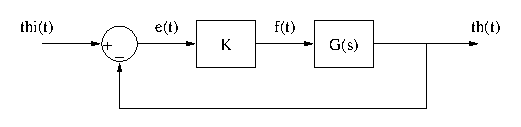
\includegraphics{propcontroller}
\end{center}
The difference between the setpoint and the measured angle is the error signal $e(t) = \theta_i(t) - \theta(t)$.  The controller in this instance just multiplies this error signal by a constant value $K$ to produce the motor current control signal $f(t)$:
\begin{equation*}
  f(t) = K e(t) = K (\theta_i(t) - \theta(t)).
\end{equation*}
In the transform domain this is $F(s) = K ( \Theta_i(s) - \Theta(s) )$.  Since $\Theta(s) = G(s) F(s)$ we have
\begin{equation*}
  \Theta(s) = K G(s) ( \Theta_i(s) - \Theta(s) ).
\end{equation*}
The closed-loop transfer function that incorporates the feedback relates the output $\Theta(s)$ to the output $\Theta_i(s)$.  From this last equation we have
\begin{equation*}
  \frac{\Theta(s)}{\Theta_i(s)} = \frac{K G(s)}{1 + K G(s)} = \frac{\frac{K}{s(s+8)}}{1 + \frac{K}{s(s+8)}}
  = \frac{K}{s^2 + 8s + K}.
\end{equation*}

The value $K$ determines how much the error signal $e(t)$ gets amplified by to produce the motor armature current $f(t)$, and it has an effect on the dynamics of the closed-loop system.  To visualise the resulting behaviour one often considers the step response of the overall system, or the output $\Theta(t)$ when the input is $\Theta_i(t) = u(t)$.   Since ${\cal L} \{ u(t) \} = 1/s$ this output will be
\begin{equation*}
  \Theta(s) = \frac{K}{s(s^2 + 8s + K)}.
\end{equation*}
Consider the case of $K=7$.  Then using partial fractions we find
\begin{equation*}
  \Theta(s) = \frac{7}{s(s^2 + 8s + 7)} = \frac{7}{s(s+1)(s+7)}
  = \frac{1}{s} - \frac{7/6}{s+1} + \frac{1/6}{s+7}.
\end{equation*}
The time-domain step response is therefore 
\begin{equation*}
  \theta(t) = (1 - 7/6 e^{-t} + 1/6 e^{-7t}) u(t).
\end{equation*}
For $K=16$ we have
\begin{equation*}
  \Theta(s) = \frac{16}{s(s^2+8s+16)} = \frac{16}{s(s+4)^2} = \frac{1}{s} - \frac{4}{(s+4)^2} - \frac{1}{s+4},
\end{equation*}
and using tables along with the frequency shift property one finds
\begin{equation*}
  \theta(t) = \left[ 1 - (1+4t) e^{-4t} \right] u(t).
\end{equation*}
For a much larger value of $K=80$ the response is
\begin{equation*}
  \Theta(s) = \frac{80}{s(s^2 + 8s + 80)} = \frac{80}{s(s+4-j8)(s+4+j8)}
  = \frac{1}{s} - \frac{s+8}{s^2+8s-80}.
\end{equation*}
Using tables of transforms this leads to the time-domain step response
\begin{equation*}
  \theta(t) = \left[ 1 - \frac{\sqrt{5}}{2} e^{-4t} \cos(8 t + \tan^{-1}(-1/2)) \right] u(t).
\end{equation*}
The three step responses calculated are shown below.
\begin{center}
  \psfrag{t}{\scriptsize $t$}
  \psfrag{th(t)}{\scriptsize $\theta(t)$}
  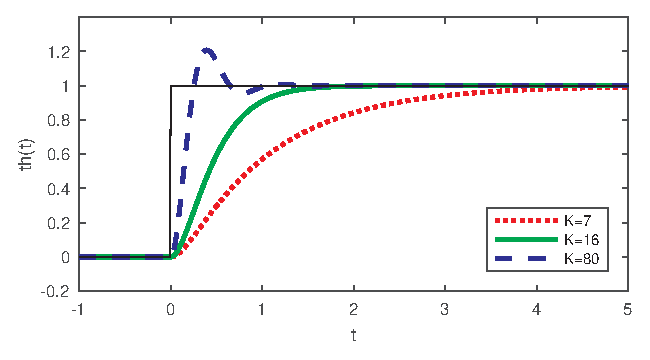
\includegraphics{stepresp2control}
\end{center}
We see that the response for $K=7$ is quite slow, and the system takes a long time to reach the setpoint.  The response for $K=80$ is much faster, but this comes at the cost of overshoot and ringing.  The case of $K=16$ yields the fastest response without oscillations.

The three cases can be distinguished by looking at the poles of the closed-loop transfer function.  These satisfy $s^2 + 8s + K=0$, or $s = -4 \pm \sqrt{16-K}$.  

For $K=7$ the two poles are real and occur at $s = -7$ and $s=-1$.  The pole at $s=-7$ leads to the term $e^{-7t}$ in the step response, which decays to zero very quickly.  The response is therefore dominated by the "slow" pole at $s=-1$, which leads to the slowly-decaying exponential term $e^{-t}$.  The system is said to be overdamped.  

For $K=16$ the poles are both at $s=-4$.  This is the case where the real poles are as far from the origin as possible, leading to the fastest response without oscillation.  The system is critically damped.

For $K=80$ the poles are complex, and occur as a conjugate pair at $s = -4 \pm 8j$.  The real part leads to exponential damping terms $e^{-4t}$ in the response, and the imaginary part determines the frequency of oscillation or ringing in the response.  The system is said to be underdamped.

In the analysis above we assumed fixed and known values for all the system components that determine $G(s)$.  In practice these might often not be completely known, or may change with time.  We can consider changes in the model to be disturbances, represented by the signals $d_i(t)$ and $d_o(t)$ below.
\begin{center}
  \psfrag{K}{\scriptsize $K$}
  \psfrag{G(s)}{\scriptsize $G(s)$}
  \psfrag{thi(t)}{\scriptsize $\theta_i(t)$}
  \psfrag{thi(t)}{\scriptsize $\theta_i(t)$}
  \psfrag{di(t)}{\scriptsize $d_i(t)$}
  \psfrag{do(t)}{\scriptsize $d_o(t)$}
  \psfrag{e(t)}{\scriptsize $e(t)$}
  \psfrag{th(t)}{\scriptsize $\theta(t)$}
  \psfrag{f(t)}{\scriptsize $f(t)$}
  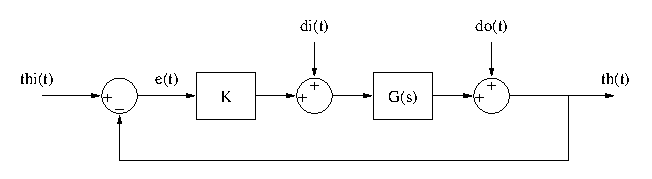
\includegraphics{propcontrollerdist}
\end{center}
In the transform domain this system satisfies
\begin{equation*}
  \Theta(s) = G(s) (K (\Theta_i(s) - \Theta(s)) + D_i(s)) + D_o(s)
\end{equation*}
This can be rearranged to
\begin{equation*}
  \Theta(s) = K G(s) \Theta_i(s) + G(s) D_i(s) + D_o(s),
\end{equation*}
so
\begin{equation*}
  \Theta(s) = \frac{K G(s)}{1 + K G(s)} \Theta_i(s) + \frac{G(s)}{1 + K G(s)} D_i(s) + \frac{1}{1 + K G(s)} D_o(s).
\end{equation*}
We observe that if $K$ is large then the last two terms will be small, and the disturbances are effectively rejected.  Thus closed-loop control can reduce the sensitivity to mismatch between the system model and the actual physical system.

This section has discussed the very simple case of a proportional controller with unity feedback.  Real control systems can be considerably more complicated.  For example, a more general controller $K(s)$ can be used, and system element could also be used in the feedback path.  The use of Laplace transforms makes it possible to deal with all of these.

\subsection{Second-order system}

Consider a second-order transfer function of the form
\begin{equation*}
  H(s) = \frac{\omega_n^2}{s^2 + 2 \zeta \omega_n s + \omega_n^2}.
\end{equation*}
The quantity $\zeta \geq 0$ is called the {\em damping ratio}, and $\omega_n$ is the {\em natural frequency}.  Using the formula for quadratic roots you can see that the poles of the system $H(s)$ satisfy $s = -\zeta \omega_n \pm \omega_n \sqrt{\zeta^2 - 1}$.

The behaviour of the system is very different depending on whether the term $\zeta^2-1$ is positive or negative.  The complicated but more interesting case occurs when $\zeta^2-1<0$, which since $\zeta$ is positive corresponds to $\zeta < 1$.  In this case the system is said to be {\em underdamped}, and the poles can be written as $s = -\zeta \omega_n \pm j \omega_n \sqrt{1 - \zeta^2}$.
\begin{center}
  \psfrag{jw}{\scriptsize $j \omega$}
  \psfrag{wn}{\scriptsize $\omega_n$}
  \psfrag{wd}{\scriptsize $\omega_d = \omega_n \sqrt{1-\zeta^2}$}
  \psfrag{sig}{\scriptsize $\sigma$}
  \psfrag{-zw}{\scriptsize $-\zeta \omega_n$}
  \psfrag{ciz}{\scriptsize $\cos^{-1} \zeta$}
  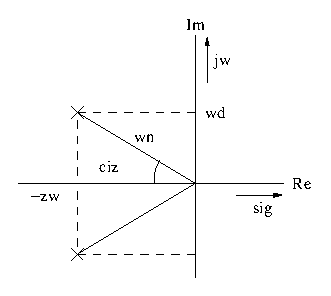
\includegraphics{pzplot2order}
\end{center}

The terminology regarding damping can be justified by considering the step response of the system, or the output when the input is $x(t) = u(t)$.  In this case $X(s) = 1/s$ and the output is given by
\begin{equation*}
  G(s) = H(s) X(s) = \frac{\omega_n^2}{s(s^2 + 2 \zeta \omega_n s + \omega_n^2)}
  = \frac{1}{s} - \frac{s + 2 \zeta \omega_n}{s^2 + 2 \zeta \omega_n s + \omega_n^2}.
\end{equation*}
This last step follows from a partial fraction expansion.  We would like to find the corresponding signal in the time domain.

One might find this inverse in a table of transforms, but it's informative to derive the response explicitly.  By completing the square the denominator can be reformulated as
\begin{equation*}
  s^2 + 2 \zeta \omega_n s + \omega_n^2 = (s + \zeta \omega_n)^2 - (\zeta \omega_n)^2 + \omega_n^2
  = (s + \zeta \omega_n)^2 + \omega_n^2 (1 - \zeta^2).
\end{equation*}
For convenience we define the quantity $\omega_d = \omega_n \sqrt{1 - \zeta^2}$, often called the {\em damped natural frequency}.  The transfer function can then be written as
\begin{equation*}
  G(s) = \frac{1}{s} - \frac{s + 2 \zeta \omega_n}{(s + \zeta \omega_n)^2 - \omega_d^2}
  = \frac{1}{s} - \frac{s + \zeta \omega_n}{(s + \zeta \omega_n)^2 + \omega_d^2} 
  - \frac{\zeta \omega_n}{(s + \zeta \omega_n)^2 + \omega_d^2}.
\end{equation*}
We split this last term into two is because it is easier to handle using standard Laplace tables.

Firstly, applying the frequency shift property to the pair $\cos(b t) u(t) \ltpair s/(s^2 + b^2)$ gives
\begin{equation*}
  e^{-at} \cos(b t) u(t) \quad \ltpair \quad \frac{(s+a)}{(s+a)^2 + b^2},
\end{equation*}
so
\begin{equation*}
  e^{-\zeta \omega_n t} \cos(\omega_d t) u(t) \quad \ltpair \quad \frac{s+\zeta \omega_n}{(s+\zeta \omega_n)^2 + \omega_d^2}.
\end{equation*}
Similarly, frequency shift applied to $\sin(b t) u(t) \ltpair b/(s^2 + b^2)$ can be used to find
\begin{equation*}
  \frac{\zeta \omega_n}{\omega_d} e^{-\zeta \omega_n t} \sin(\omega_d t) u(t) \quad \ltpair \quad 
  \frac{\zeta \omega_n}{(s+\zeta \omega_n)^2 + \omega_d^2}
\end{equation*}
The step response can then be found as the inverse Laplace transform:
\begin{align*}
  g(t) &= \left[ 1 - e^{-\zeta \omega_n t} \cos(\omega_d t) 
  - \frac{\zeta \omega_n}{\omega_d} e^{-\zeta \omega_n t} \sin(\omega_d t) \right] u(t) \\
  &= \left[ 1 - e^{-\zeta \omega_n t} \cos(\omega_d t) 
  - \frac{\zeta}{\sqrt{1 - \zeta^2}} e^{-\zeta \omega_n t} \sin(\omega_d t) \right] u(t) \\
  &= \left[ 1 - \frac{e^{-\zeta \omega_n t} }{\sqrt{1 - \zeta^2}} \left( \sqrt{1 - \zeta^2} \cos(\omega_d t) 
  + \zeta \sin(\omega_d t) \right) \right] u(t).
\end{align*}
If we let $\zeta = \cos(\theta)$ and note that $\sqrt{1 - \zeta^2} = \sin(\theta)$, this can be written as
\begin{equation*}
  g(t) = \left[ 1 - \frac{e^{-\zeta \omega_n t} }{\sqrt{1 - \zeta^2}} \left( \sin(\theta) \cos(\omega_d t) 
  + \cos(\theta) \sin(\omega_d t) \right) \right] u(t).
\end{equation*}
When $\theta=0$ then the inner term in brackets is just $\sin(\omega_d t)$, when $\theta=1$ it is $\cos(\omega_d t)$, and for $\theta$ in between it's a combination of the two.  The step response can finally be written as
\begin{equation*}
  g(t) = \left[ 1 - \frac{e^{-\zeta \omega_n t} }{\sqrt{1 - \zeta^2}} \sin(\omega_d t + \theta) \right] u(t)
\end{equation*}
since $\sin(a+b) = \sin a \cos b + \cos a \sin b$, where $\theta = \cos^{-1}(\zeta)$.

Plots of the step response for $\omega_n=1$ and three different values of $\zeta$ are shown below.
\begin{center}
  \psfrag{t}{\scriptsize $t$}
  \psfrag{zeta=0.99}{\scriptsize $\zeta=0.99$}
  \psfrag{zeta=0.5}{\scriptsize $\zeta=0.5$}
  \psfrag{zeta=0.1}{\scriptsize $\zeta=0.1$}
  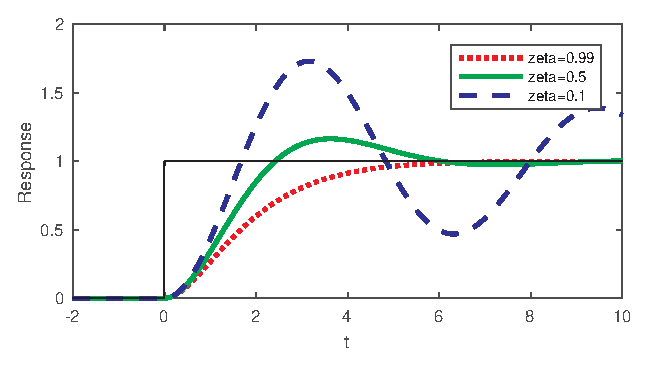
\includegraphics{stepresp2underd}
\end{center}
As the damping factor tends towards zero the response rises more steeply but exhibits overshoot and becomes more oscillatory.  This is sometimes known as {\em ringing}.

The system is {\em overdamped} when $\zeta^2-1>0$, or $\zeta>1$.  In this case there are two real poles at $s = -\zeta \omega_n \pm \omega_n \sqrt{\zeta^2 - 1}$, and the step response consists of two exponential terms with no oscillation.  If one of the poles is much closer to the origin than the other then the response is dominated by this slower pole.

{\em Find\marginpar{\bf Exercise:} and plot the step response of an overdamped second order system for $\omega_n=1$ and $\zeta = 2, 4, 8$.

\subsection{Stability}

Lathi section 6.7-6.

\end{document}
